\documentclass[twoside]{book}

% Packages required by doxygen
\usepackage{fixltx2e}
\usepackage{calc}
\usepackage{doxygen}
\usepackage{graphicx}
\usepackage[utf8]{inputenc}
\usepackage{makeidx}
\usepackage{multicol}
\usepackage{multirow}
\PassOptionsToPackage{warn}{textcomp}
\usepackage{textcomp}
\usepackage[nointegrals]{wasysym}
\usepackage[table]{xcolor}

% NLS support packages
\usepackage[spanish]{babel}
% Font selection
\usepackage[T1]{fontenc}
\usepackage{mathptmx}
\usepackage[scaled=.90]{helvet}
\usepackage{courier}
\usepackage{amssymb}
\usepackage{sectsty}
\renewcommand{\familydefault}{\sfdefault}
\allsectionsfont{%
  \fontseries{bc}\selectfont%
  \color{darkgray}%
}
\renewcommand{\DoxyLabelFont}{%
  \fontseries{bc}\selectfont%
  \color{darkgray}%
}
\newcommand{\+}{\discretionary{\mbox{\scriptsize$\hookleftarrow$}}{}{}}

% Page & text layout
\usepackage{geometry}
\geometry{%
  letterpaper,%
  top=2.5cm,%
  bottom=2.5cm,%
  left=2.5cm,%
  right=2.5cm%
}
\tolerance=750
\hfuzz=15pt
\hbadness=750
\setlength{\emergencystretch}{15pt}
\setlength{\parindent}{0cm}
\setlength{\parskip}{0.2cm}
\makeatletter
\renewcommand{\paragraph}{%
  \@startsection{paragraph}{4}{0ex}{-1.0ex}{1.0ex}{%
    \normalfont\normalsize\bfseries\SS@parafont%
  }%
}
\renewcommand{\subparagraph}{%
  \@startsection{subparagraph}{5}{0ex}{-1.0ex}{1.0ex}{%
    \normalfont\normalsize\bfseries\SS@subparafont%
  }%
}
\makeatother

% Headers & footers
\usepackage{fancyhdr}
\pagestyle{fancyplain}
\fancyhead[LE]{\fancyplain{}{\bfseries\thepage}}
\fancyhead[CE]{\fancyplain{}{}}
\fancyhead[RE]{\fancyplain{}{\bfseries\leftmark}}
\fancyhead[LO]{\fancyplain{}{\bfseries\rightmark}}
\fancyhead[CO]{\fancyplain{}{}}
\fancyhead[RO]{\fancyplain{}{\bfseries\thepage}}
\fancyfoot[LE]{\fancyplain{}{}}
\fancyfoot[CE]{\fancyplain{}{}}
\fancyfoot[RE]{\fancyplain{}{\bfseries\scriptsize Generado el Jueves, 19 de Enero de 2017 23\+:10\+:13 para image\+Server por Doxygen }}
\fancyfoot[LO]{\fancyplain{}{\bfseries\scriptsize Generado el Jueves, 19 de Enero de 2017 23\+:10\+:13 para image\+Server por Doxygen }}
\fancyfoot[CO]{\fancyplain{}{}}
\fancyfoot[RO]{\fancyplain{}{}}
\renewcommand{\footrulewidth}{0.4pt}
\renewcommand{\chaptermark}[1]{%
  \markboth{#1}{}%
}
\renewcommand{\sectionmark}[1]{%
  \markright{\thesection\ #1}%
}

% Indices & bibliography
\usepackage{natbib}
\usepackage[titles]{tocloft}
\setcounter{tocdepth}{3}
\setcounter{secnumdepth}{5}
\makeindex

% Hyperlinks (required, but should be loaded last)
\usepackage{ifpdf}
\ifpdf
  \usepackage[pdftex,pagebackref=true]{hyperref}
\else
  \usepackage[ps2pdf,pagebackref=true]{hyperref}
\fi
\hypersetup{%
  colorlinks=true,%
  linkcolor=blue,%
  citecolor=blue,%
  unicode%
}

% Custom commands
\newcommand{\clearemptydoublepage}{%
  \newpage{\pagestyle{empty}\cleardoublepage}%
}


%===== C O N T E N T S =====

\begin{document}

% Titlepage & ToC
\hypersetup{pageanchor=false,
             bookmarks=true,
             bookmarksnumbered=true,
             pdfencoding=unicode
            }
\pagenumbering{roman}
\begin{titlepage}
\vspace*{7cm}
\begin{center}%
{\Large image\+Server \\[1ex]\large 1.\+0 }\\
\vspace*{1cm}
{\large Generado por Doxygen 1.8.8}\\
\vspace*{0.5cm}
{\small Jueves, 19 de Enero de 2017 23:10:13}\\
\end{center}
\end{titlepage}
\clearemptydoublepage
\tableofcontents
\clearemptydoublepage
\pagenumbering{arabic}
\hypersetup{pageanchor=true}

%--- Begin generated contents ---
\chapter{image\+Server}
\label{md_README}
\hypertarget{md_README}{}
An open\+C\+V image server, to distribute captured image to multiple clients. 
\chapter{Indice de namespaces}
\section{Lista de 'namespaces'}
Lista de los 'namespaces', con una breve descripción\+:\begin{DoxyCompactList}
\item\contentsline{section}{\hyperlink{namespaceremoteFrame}{remote\+Frame} }{\pageref{namespaceremoteFrame}}{}
\item\contentsline{section}{\hyperlink{namespacetestClient}{test\+Client} }{\pageref{namespacetestClient}}{}
\end{DoxyCompactList}

\chapter{Indice jerárquico}
\input{hierarchy}
\chapter{Índice de clases}
\section{Lista de clases}
Lista de las clases, estructuras, uniones e interfaces con una breve descripción\+:\begin{DoxyCompactList}
\item\contentsline{section}{\hyperlink{classCamera}{Camera} \\*Esta clase permite capturar imágenes de una cámara, utilizando los métodos provisto por la biblioteca highgui. Las imagenes capturadas son almacenadas en una cola. Se proveen mecanismos de sincronización para el acceso concurrente a dicha cola }{\pageref{classCamera}}{}
\item\contentsline{section}{\hyperlink{classclass}{class} \\*Esta clase crea un \char`\"{}stream socket\char`\"{} y lo asocia a una direccion I\+P y un puerto, y provee servicios básicos para atender de manera concurrente a multiples clientes }{\pageref{classclass}}{}
\item\contentsline{section}{\hyperlink{classClient}{Client} \\*Esta clase crea un objeto que permite conectarse via un socket con un servidor, para transmitir información }{\pageref{classClient}}{}
\item\contentsline{section}{\hyperlink{classConnServer}{Conn\+Server} }{\pageref{classConnServer}}{}
\item\contentsline{section}{\hyperlink{structcornerData}{corner\+Data} \\*Esta estructura contiene información de esquinas que se utiliza durante la captura de posiciones en la pantalla usando el raton }{\pageref{structcornerData}}{}
\item\contentsline{section}{\hyperlink{classImageBuffer}{Image\+Buffer} \\*Esta clase especializa la clase Ringbuffer para operar on objetos de tipo \hyperlink{structinfoFrame}{info\+Frame}. Aparte añade dos métodos nuevos\+: get\+Last y adv\+Head }{\pageref{classImageBuffer}}{}
\item\contentsline{section}{\hyperlink{structImageInfo}{Image\+Info} \\*Esta clase define la estructura Imagen\+Info, que define el encabezado que se utiliza para la transmisión de imagenes }{\pageref{structImageInfo}}{}
\item\contentsline{section}{\hyperlink{classImageServer}{Image\+Server} \\*Objetos instanciados de esta clase, capturan imágenes de una cámara y las almacena en un buffer, y permite la conexión via sockets de clientes a quienes provee de dichas imágenes }{\pageref{classImageServer}}{}
\item\contentsline{section}{\hyperlink{structinfoFrame}{info\+Frame} \\*Objetos instanciados a partir de esta estructura almacenan una imagen utilizando un objeto cv\+::\+Mat y el tiempo en que fue capturada (un 'timestamp') }{\pageref{structinfoFrame}}{}
\item\contentsline{section}{\hyperlink{classremoteFrame_1_1remoteFrame}{remote\+Frame} }{\pageref{classremoteFrame_1_1remoteFrame}}{}
\item\contentsline{section}{\hyperlink{classRingBuffer}{Ring\+Buffer$<$ X $>$} \\*Esta clase implementa un contador modular. El objeto funciona como un entero, que aritmeticamente opera usando aritmética modular }{\pageref{classRingBuffer}}{}
\item\contentsline{section}{\hyperlink{classRingCounter}{Ring\+Counter} }{\pageref{classRingCounter}}{}
\item\contentsline{section}{\hyperlink{classtemplate}{template} \\*Esta clase define una cola finita a partir de un arreglo. Depende del objeto \hyperlink{classRingCounter}{Ring\+Counter} para manejar indices circulares. La clase se construye como un plantilla, y se espera que los objetos quw consitituyan la cola tengan sobrecargado el operador de copia. La clase provee métodos para añadir un objeto al final de la cola, sacar del frente de la cola. La clase cuenta con pthread\+\_\+mutexes para sincronizar acceso cuando se utiliza en un ambiente multihebras }{\pageref{classtemplate}}{}
\end{DoxyCompactList}

\chapter{Indice de archivos}
\section{Lista de archivos}
Lista de todos los archivos con descripciones breves\+:\begin{DoxyCompactList}
\item\contentsline{section}{\hyperlink{imgServer_8cpp}{img\+Server.\+cpp} }{\pageref{imgServer_8cpp}}{}
\item\contentsline{section}{\hyperlink{remoteFrame_8py}{remote\+Frame.\+py} }{\pageref{remoteFrame_8py}}{}
\item\contentsline{section}{\hyperlink{testClient_8cpp}{test\+Client.\+cpp} }{\pageref{testClient_8cpp}}{}
\item\contentsline{section}{\hyperlink{testClient_8py}{test\+Client.\+py} }{\pageref{testClient_8py}}{}
\item\contentsline{section}{include/\hyperlink{Camera_8h}{Camera.\+h} \\*Archivo de encabezado donde se define la clase \hyperlink{classCamera}{Camera}. Esta Clase tiene como función capturar imágenes una camara. Cada cuadro capturado se almacena en una cola, para que pueda ser procesados posteriormente }{\pageref{Camera_8h}}{}
\item\contentsline{section}{include/\hyperlink{Client_8h}{Client.\+h} \\*En este archivo de encabezado se define la clase \hyperlink{classClient}{Client}. Dicha clase crea al ser instanciada un objeto que facilita la parte cliente de un sistema de comunicación basado en sockets }{\pageref{Client_8h}}{}
\item\contentsline{section}{include/\hyperlink{ConnServer_8h}{Conn\+Server.\+h} }{\pageref{ConnServer_8h}}{}
\item\contentsline{section}{include/\hyperlink{imageBuffer_8h}{image\+Buffer.\+h} }{\pageref{imageBuffer_8h}}{}
\item\contentsline{section}{include/\hyperlink{ImageServer_8h}{Image\+Server.\+h} \\*Este archivo contiene las definición de la clase \hyperlink{classImageServer}{Image\+Server}. Objetos instanciados de esta clase capturan imágenes de una cámara, y los ofrecen a traves de un socket a clientes que se conectan a el. Ademas provee capacidades, para transformar la imagenes capturadas (homografias), y mezclar éstas con imagenes predefinidas }{\pageref{ImageServer_8h}}{}
\item\contentsline{section}{include/\hyperlink{infoFrame_8h}{info\+Frame.\+h} \\*En este archivo se encuentra la defincion de la estructura \hyperlink{structinfoFrame}{info\+Frame}, que se utiliza para almacenar una imagen junto con el tiempo en que fue capturada }{\pageref{infoFrame_8h}}{}
\item\contentsline{section}{include/\hyperlink{RingBuffer_8h}{Ring\+Buffer.\+h} \\*Archivo de encabezado en donde se define ela clase \hyperlink{classRingBuffer}{Ring\+Buffer} }{\pageref{RingBuffer_8h}}{}
\item\contentsline{section}{include/\hyperlink{RingCounter_8h}{Ring\+Counter.\+h} \\*Este archivo contiene la definición de un contador módular }{\pageref{RingCounter_8h}}{}
\item\contentsline{section}{include/\hyperlink{SockIO_8h}{Sock\+I\+O.\+h} \\*En este archivo de encabezado se definen dos funciones que permiten enviar y recibir una cantidad arbitrariamente grande de datos a través de un socket }{\pageref{SockIO_8h}}{}
\item\contentsline{section}{include/\hyperlink{structures_8h}{structures.\+h} \\*En este archivo se define la estructura \hyperlink{structImageInfo}{Image\+Info}, que se utiliza en el servidor de imagenes, así como se definen varios valores por defecto }{\pageref{structures_8h}}{}
\item\contentsline{section}{src/\hyperlink{Camera_8cpp}{Camera.\+cpp} \\*Este archivo contiene el código que de los métodos de la clase Camara }{\pageref{Camera_8cpp}}{}
\item\contentsline{section}{src/\hyperlink{Client_8cpp}{Client.\+cpp} \\*Este archivo contiene el código que de los métodos de la clase \hyperlink{classClient}{Client} }{\pageref{Client_8cpp}}{}
\item\contentsline{section}{src/\hyperlink{ConnServer_8cpp}{Conn\+Server.\+cpp} \\*Este archivo contiene el código que de los métodos de la clase \hyperlink{ConnServer_8cpp}{Conn\+Server.\+cpp} }{\pageref{ConnServer_8cpp}}{}
\item\contentsline{section}{src/\hyperlink{ImageServer_8cpp}{Image\+Server.\+cpp} }{\pageref{ImageServer_8cpp}}{}
\item\contentsline{section}{src/\hyperlink{SockIO_8cpp}{Sock\+I\+O.\+cpp} \\*Este archivo contiene el código que de los funciones Read y Write definidias en \hyperlink{SockIO_8h}{Sock\+I\+O.\+h} }{\pageref{SockIO_8cpp}}{}
\end{DoxyCompactList}

\chapter{Documentación de namespaces}
\hypertarget{namespaceremoteFrame}{\section{Referencia del Namespace remote\+Frame}
\label{namespaceremoteFrame}\index{remote\+Frame@{remote\+Frame}}
}
\subsection*{Clases}
\begin{DoxyCompactItemize}
\item 
class \hyperlink{classremoteFrame_1_1remoteFrame}{remote\+Frame}
\end{DoxyCompactItemize}

\hypertarget{namespacetestClient}{\section{Referencia del Namespace test\+Client}
\label{namespacetestClient}\index{test\+Client@{test\+Client}}
}
\subsection*{Variables}
\begin{DoxyCompactItemize}
\item 
string \hyperlink{namespacetestClient_aa723f31c9553b9750fa5b98615d0a8af}{address} = '127.\+0.\+0.\+1'
\item 
tuple \hyperlink{namespacetestClient_aad55a8f6b73a60a17d26dfc0d628f89a}{argc} = len(sys.\+argv)
\item 
tuple \hyperlink{namespacetestClient_aec8b285f81ee0dc468a6b86b4345e127}{img} = r\+F.\+get\+Frame()
\item 
\hyperlink{namespacetestClient_a09ad76b7b5cee406ff62ac1cdda80c27}{Mask} = None
\item 
int \hyperlink{namespacetestClient_a1aadf525515ecfcf662c2aa51a503763}{port} = 8888
\item 
tuple \hyperlink{namespacetestClient_a0be24333dfe323a6c01b9f452cc8b142}{r\+F} = \hyperlink{classremoteFrame_1_1remoteFrame}{remote\+Frame}(\hyperlink{namespacetestClient_aa723f31c9553b9750fa5b98615d0a8af}{address}, \hyperlink{namespacetestClient_a1aadf525515ecfcf662c2aa51a503763}{port}, \hyperlink{namespacetestClient_a09ad76b7b5cee406ff62ac1cdda80c27}{Mask})
\end{DoxyCompactItemize}


\subsection{Documentación de las variables}
\hypertarget{namespacetestClient_aa723f31c9553b9750fa5b98615d0a8af}{\index{test\+Client@{test\+Client}!address@{address}}
\index{address@{address}!test\+Client@{test\+Client}}
\subsubsection[{address}]{\setlength{\rightskip}{0pt plus 5cm}list address = '127.\+0.\+0.\+1'}}\label{namespacetestClient_aa723f31c9553b9750fa5b98615d0a8af}


Definición en la línea 10 del archivo test\+Client.\+py.

\hypertarget{namespacetestClient_aad55a8f6b73a60a17d26dfc0d628f89a}{\index{test\+Client@{test\+Client}!argc@{argc}}
\index{argc@{argc}!test\+Client@{test\+Client}}
\subsubsection[{argc}]{\setlength{\rightskip}{0pt plus 5cm}tuple argc = len(sys.\+argv)}}\label{namespacetestClient_aad55a8f6b73a60a17d26dfc0d628f89a}


Definición en la línea 13 del archivo test\+Client.\+py.

\hypertarget{namespacetestClient_aec8b285f81ee0dc468a6b86b4345e127}{\index{test\+Client@{test\+Client}!img@{img}}
\index{img@{img}!test\+Client@{test\+Client}}
\subsubsection[{img}]{\setlength{\rightskip}{0pt plus 5cm}tuple img = r\+F.\+get\+Frame()}}\label{namespacetestClient_aec8b285f81ee0dc468a6b86b4345e127}


Definición en la línea 26 del archivo test\+Client.\+py.

\hypertarget{namespacetestClient_a09ad76b7b5cee406ff62ac1cdda80c27}{\index{test\+Client@{test\+Client}!Mask@{Mask}}
\index{Mask@{Mask}!test\+Client@{test\+Client}}
\subsubsection[{Mask}]{\setlength{\rightskip}{0pt plus 5cm}tuple Mask = None}}\label{namespacetestClient_a09ad76b7b5cee406ff62ac1cdda80c27}


Definición en la línea 11 del archivo test\+Client.\+py.

\hypertarget{namespacetestClient_a1aadf525515ecfcf662c2aa51a503763}{\index{test\+Client@{test\+Client}!port@{port}}
\index{port@{port}!test\+Client@{test\+Client}}
\subsubsection[{port}]{\setlength{\rightskip}{0pt plus 5cm}tuple port = 8888}}\label{namespacetestClient_a1aadf525515ecfcf662c2aa51a503763}


Definición en la línea 9 del archivo test\+Client.\+py.

\hypertarget{namespacetestClient_a0be24333dfe323a6c01b9f452cc8b142}{\index{test\+Client@{test\+Client}!r\+F@{r\+F}}
\index{r\+F@{r\+F}!test\+Client@{test\+Client}}
\subsubsection[{r\+F}]{\setlength{\rightskip}{0pt plus 5cm}tuple r\+F = {\bf remote\+Frame}({\bf address}, {\bf port}, {\bf Mask})}}\label{namespacetestClient_a0be24333dfe323a6c01b9f452cc8b142}


Definición en la línea 21 del archivo test\+Client.\+py.


\chapter{Documentación de las clases}
\input{classCamera}
\input{classclass}
\input{classClient}
\input{classConnServer}
\hypertarget{structcornerData}{\section{Referencia de la Estructura corner\+Data}
\label{structcornerData}\index{corner\+Data@{corner\+Data}}
}


Esta estructura contiene información de esquinas que se utiliza durante la captura de posiciones en la pantalla usando el raton.  


\subsection*{Métodos públicos}
\begin{DoxyCompactItemize}
\item 
\hyperlink{structcornerData_a9f4acaee1021cd3fae7619a520f2da33}{corner\+Data} ()
\begin{DoxyCompactList}\small\item\em Constructor del objeto. \end{DoxyCompactList}\end{DoxyCompactItemize}
\subsection*{Atributos públicos}
\begin{DoxyCompactItemize}
\item 
int \hyperlink{structcornerData_a961800bf60ff693820efbf7f4bc72788}{cont}
\begin{DoxyCompactList}\small\item\em Contador. \end{DoxyCompactList}\item 
Point2f \hyperlink{structcornerData_a6d9e631d38806edbc61499fd4794baea}{crn} \mbox{[}4\mbox{]}
\begin{DoxyCompactList}\small\item\em Arreglo de 4 objetos tipo Point2f en donde se almacenaran las esquinas. \end{DoxyCompactList}\end{DoxyCompactItemize}


\subsection{Descripción detallada}
Esta estructura contiene información de esquinas que se utiliza durante la captura de posiciones en la pantalla usando el raton. 

Definición en la línea 33 del archivo img\+Server.\+cpp.



\subsection{Documentación del constructor y destructor}
\hypertarget{structcornerData_a9f4acaee1021cd3fae7619a520f2da33}{\index{corner\+Data@{corner\+Data}!corner\+Data@{corner\+Data}}
\index{corner\+Data@{corner\+Data}!corner\+Data@{corner\+Data}}
\subsubsection[{corner\+Data}]{\setlength{\rightskip}{0pt plus 5cm}{\bf corner\+Data} (
\begin{DoxyParamCaption}
{}
\end{DoxyParamCaption}
)\hspace{0.3cm}{\ttfamily [inline]}}}\label{structcornerData_a9f4acaee1021cd3fae7619a520f2da33}


Constructor del objeto. 



Definición en la línea 42 del archivo img\+Server.\+cpp.


\begin{DoxyCode}
43     \{
44         \hyperlink{structcornerData_a961800bf60ff693820efbf7f4bc72788}{cont} = 0;
45     \}
\end{DoxyCode}


\subsection{Documentación de los datos miembro}
\hypertarget{structcornerData_a961800bf60ff693820efbf7f4bc72788}{\index{corner\+Data@{corner\+Data}!cont@{cont}}
\index{cont@{cont}!corner\+Data@{corner\+Data}}
\subsubsection[{cont}]{\setlength{\rightskip}{0pt plus 5cm}int cont}}\label{structcornerData_a961800bf60ff693820efbf7f4bc72788}


Contador. 



Definición en la línea 36 del archivo img\+Server.\+cpp.

\hypertarget{structcornerData_a6d9e631d38806edbc61499fd4794baea}{\index{corner\+Data@{corner\+Data}!crn@{crn}}
\index{crn@{crn}!corner\+Data@{corner\+Data}}
\subsubsection[{crn}]{\setlength{\rightskip}{0pt plus 5cm}Point2f crn\mbox{[}4\mbox{]}}}\label{structcornerData_a6d9e631d38806edbc61499fd4794baea}


Arreglo de 4 objetos tipo Point2f en donde se almacenaran las esquinas. 



Definición en la línea 35 del archivo img\+Server.\+cpp.



La documentación para esta estructura fue generada a partir del siguiente fichero\+:\begin{DoxyCompactItemize}
\item 
\hyperlink{imgServer_8cpp}{img\+Server.\+cpp}\end{DoxyCompactItemize}

\input{classImageBuffer}
\input{structImageInfo}
\input{classImageServer}
\input{structinfoFrame}
\hypertarget{classremoteFrame_1_1remoteFrame}{\section{Referencia de la Clase remote\+Frame}
\label{classremoteFrame_1_1remoteFrame}\index{remote\+Frame@{remote\+Frame}}
}
\subsection*{Métodos públicos}
\begin{DoxyCompactItemize}
\item 
def \hyperlink{classremoteFrame_1_1remoteFrame_ac775ee34451fdfa742b318538164070e}{\+\_\+\+\_\+init\+\_\+\+\_\+}
\item 
def \hyperlink{classremoteFrame_1_1remoteFrame_afa251912978c7d5ccf7e5a027a4d12ee}{\+\_\+\+\_\+del\+\_\+\+\_\+}
\item 
def \hyperlink{classremoteFrame_1_1remoteFrame_af9458ce42581fff9b03a7e20c1e333d0}{get\+Frame}
\end{DoxyCompactItemize}
\subsection*{Atributos públicos}
\begin{DoxyCompactItemize}
\item 
\hyperlink{classremoteFrame_1_1remoteFrame_ade5a18d52133ef21f211020ceb464c07}{address}
\item 
\hyperlink{classremoteFrame_1_1remoteFrame_a60d28e417cda8ed5b817c14e537c5629}{cl}
\item 
\hyperlink{classremoteFrame_1_1remoteFrame_a291536e8bf5e2f42dec8ed3f82b13487}{Mask}
\item 
\hyperlink{classremoteFrame_1_1remoteFrame_a643996cc8d402d1005166f956adfe0da}{msg\+Length}
\item 
\hyperlink{classremoteFrame_1_1remoteFrame_af8fb0f45ee0195c7422a49e6a8d72369}{port}
\item 
\hyperlink{classremoteFrame_1_1remoteFrame_aec4a6f499c74a3d34d4dfe9930c9e115}{where}
\end{DoxyCompactItemize}


\subsection{Descripción detallada}


Definición en la línea 8 del archivo remote\+Frame.\+py.



\subsection{Documentación del constructor y destructor}
\hypertarget{classremoteFrame_1_1remoteFrame_ac775ee34451fdfa742b318538164070e}{\index{remote\+Frame\+::remote\+Frame@{remote\+Frame\+::remote\+Frame}!\+\_\+\+\_\+init\+\_\+\+\_\+@{\+\_\+\+\_\+init\+\_\+\+\_\+}}
\index{\+\_\+\+\_\+init\+\_\+\+\_\+@{\+\_\+\+\_\+init\+\_\+\+\_\+}!remote\+Frame\+::remote\+Frame@{remote\+Frame\+::remote\+Frame}}
\subsubsection[{\+\_\+\+\_\+init\+\_\+\+\_\+}]{\setlength{\rightskip}{0pt plus 5cm}def \+\_\+\+\_\+init\+\_\+\+\_\+ (
\begin{DoxyParamCaption}
\item[{}]{self, }
\item[{}]{address = {\ttfamily '127.0.0.1'}, }
\item[{}]{port = {\ttfamily 8888}, }
\item[{}]{Mask = {\ttfamily None}}
\end{DoxyParamCaption}
)}}\label{classremoteFrame_1_1remoteFrame_ac775ee34451fdfa742b318538164070e}


Definición en la línea 9 del archivo remote\+Frame.\+py.


\begin{DoxyCode}
9 
10     \textcolor{keyword}{def }\hyperlink{classremoteFrame_1_1remoteFrame_ac775ee34451fdfa742b318538164070e}{\_\_init\_\_}(self, address='127.0.0.1', port=8888, Mask=None):
11         self.\hyperlink{classremoteFrame_1_1remoteFrame_ade5a18d52133ef21f211020ceb464c07}{address} = address
12         self.\hyperlink{classremoteFrame_1_1remoteFrame_af8fb0f45ee0195c7422a49e6a8d72369}{port} = port
13         self.\hyperlink{classremoteFrame_1_1remoteFrame_a60d28e417cda8ed5b817c14e537c5629}{cl} = socket.socket(socket.AF\_INET, socket.SOCK\_STREAM)
14         self.cl.connect((self.\hyperlink{classremoteFrame_1_1remoteFrame_ade5a18d52133ef21f211020ceb464c07}{address}, self.\hyperlink{classremoteFrame_1_1remoteFrame_af8fb0f45ee0195c7422a49e6a8d72369}{port}))
15         self.\hyperlink{classremoteFrame_1_1remoteFrame_a643996cc8d402d1005166f956adfe0da}{msgLength} = 10
16         \textcolor{keywordflow}{if} Mask != \textcolor{keywordtype}{None}:
17             b, g, r = cv2.split(Mask)
18             self.\hyperlink{classremoteFrame_1_1remoteFrame_aec4a6f499c74a3d34d4dfe9930c9e115}{where} = b & 255
19             self.\hyperlink{classremoteFrame_1_1remoteFrame_aec4a6f499c74a3d34d4dfe9930c9e115}{where} &= g & 255
20             self.\hyperlink{classremoteFrame_1_1remoteFrame_aec4a6f499c74a3d34d4dfe9930c9e115}{where} &= r & 255
21             self.\hyperlink{classremoteFrame_1_1remoteFrame_aec4a6f499c74a3d34d4dfe9930c9e115}{where} = 255-self.\hyperlink{classremoteFrame_1_1remoteFrame_aec4a6f499c74a3d34d4dfe9930c9e115}{where}
22             self.\hyperlink{classremoteFrame_1_1remoteFrame_aec4a6f499c74a3d34d4dfe9930c9e115}{where} = 255 - self.\hyperlink{classremoteFrame_1_1remoteFrame_aec4a6f499c74a3d34d4dfe9930c9e115}{where}
23             self.\hyperlink{classremoteFrame_1_1remoteFrame_aec4a6f499c74a3d34d4dfe9930c9e115}{where}=cv2.merge((self.\hyperlink{classremoteFrame_1_1remoteFrame_aec4a6f499c74a3d34d4dfe9930c9e115}{where},self.\hyperlink{classremoteFrame_1_1remoteFrame_aec4a6f499c74a3d34d4dfe9930c9e115}{where},self.
      \hyperlink{classremoteFrame_1_1remoteFrame_aec4a6f499c74a3d34d4dfe9930c9e115}{where}))
24             self.\hyperlink{classremoteFrame_1_1remoteFrame_a291536e8bf5e2f42dec8ed3f82b13487}{Mask} = Mask & ~self.\hyperlink{classremoteFrame_1_1remoteFrame_aec4a6f499c74a3d34d4dfe9930c9e115}{where}
25         \textcolor{keywordflow}{else}:
            self.\hyperlink{classremoteFrame_1_1remoteFrame_a291536e8bf5e2f42dec8ed3f82b13487}{Mask} = \textcolor{keywordtype}{None}
\end{DoxyCode}
\hypertarget{classremoteFrame_1_1remoteFrame_afa251912978c7d5ccf7e5a027a4d12ee}{\index{remote\+Frame\+::remote\+Frame@{remote\+Frame\+::remote\+Frame}!\+\_\+\+\_\+del\+\_\+\+\_\+@{\+\_\+\+\_\+del\+\_\+\+\_\+}}
\index{\+\_\+\+\_\+del\+\_\+\+\_\+@{\+\_\+\+\_\+del\+\_\+\+\_\+}!remote\+Frame\+::remote\+Frame@{remote\+Frame\+::remote\+Frame}}
\subsubsection[{\+\_\+\+\_\+del\+\_\+\+\_\+}]{\setlength{\rightskip}{0pt plus 5cm}def \+\_\+\+\_\+del\+\_\+\+\_\+ (
\begin{DoxyParamCaption}
\item[{}]{self}
\end{DoxyParamCaption}
)}}\label{classremoteFrame_1_1remoteFrame_afa251912978c7d5ccf7e5a027a4d12ee}


Definición en la línea 26 del archivo remote\+Frame.\+py.


\begin{DoxyCode}
26 
27     \textcolor{keyword}{def }\hyperlink{classremoteFrame_1_1remoteFrame_afa251912978c7d5ccf7e5a027a4d12ee}{\_\_del\_\_} (self):
28         msg=\textcolor{stringliteral}{"QUIT      "}
29         self.cl.sendall(msg)
30         msg = self.cl.recv(10)
31         \textcolor{keywordflow}{if} msg[:3] != \textcolor{stringliteral}{"BYE"}:
32             \textcolor{keywordflow}{print} \textcolor{stringliteral}{'No se recibió "BYE" :-(, se recibió |'}+msg+\textcolor{stringliteral}{'| '}
33         \textcolor{keywordflow}{else}:
            \textcolor{keywordflow}{print} \textcolor{stringliteral}{'remoteFrame: Cerrando conexión'}
\end{DoxyCode}


\subsection{Documentación de las funciones miembro}
\hypertarget{classremoteFrame_1_1remoteFrame_af9458ce42581fff9b03a7e20c1e333d0}{\index{remote\+Frame\+::remote\+Frame@{remote\+Frame\+::remote\+Frame}!get\+Frame@{get\+Frame}}
\index{get\+Frame@{get\+Frame}!remote\+Frame\+::remote\+Frame@{remote\+Frame\+::remote\+Frame}}
\subsubsection[{get\+Frame}]{\setlength{\rightskip}{0pt plus 5cm}def get\+Frame (
\begin{DoxyParamCaption}
\item[{}]{self}
\end{DoxyParamCaption}
)}}\label{classremoteFrame_1_1remoteFrame_af9458ce42581fff9b03a7e20c1e333d0}


Definición en la línea 34 del archivo remote\+Frame.\+py.


\begin{DoxyCode}
34 
35     \textcolor{keyword}{def }\hyperlink{classremoteFrame_1_1remoteFrame_af9458ce42581fff9b03a7e20c1e333d0}{getFrame}(self):
36         msg=\textcolor{stringliteral}{"IMG       "}
37         self.cl.sendall(msg)
38         msg = self.cl.recv(16)
39         msgb = map(ord, msg)
40         rows =(msgb[1]<<8)+msgb[0]+(((msgb[3]<<8)+msgb[2])<<16)
41         cols =(msgb[5]<<8)+msgb[4]+(((msgb[7]<<8)+msgb[6])<<16)
42         itype =(msgb[9]<<8)+msgb[8]+(((msgb[11]<<8)+msgb[10])<<16)
43         size =(msgb[13]<<8)+msgb[12]+(((msgb[15]<<8)+msgb[14])<<16)
44         recibidos = size
45         img=[]
46         \textcolor{keywordflow}{while} (recibidos != 0):
47             buff = self.cl.recv(recibidos)
48             recibidos -= len(buff)
49             img += buff
50         I=np.array(bytearray(img)).reshape(rows,cols,3)
51         \textcolor{keywordflow}{if} self.\hyperlink{classremoteFrame_1_1remoteFrame_a291536e8bf5e2f42dec8ed3f82b13487}{Mask} != \textcolor{keywordtype}{None}:
52             I = (I & self.\hyperlink{classremoteFrame_1_1remoteFrame_aec4a6f499c74a3d34d4dfe9930c9e115}{where}) + self.\hyperlink{classremoteFrame_1_1remoteFrame_a291536e8bf5e2f42dec8ed3f82b13487}{Mask}
53 
54         \textcolor{keywordflow}{return} I
\end{DoxyCode}


\subsection{Documentación de los datos miembro}
\hypertarget{classremoteFrame_1_1remoteFrame_ade5a18d52133ef21f211020ceb464c07}{\index{remote\+Frame\+::remote\+Frame@{remote\+Frame\+::remote\+Frame}!address@{address}}
\index{address@{address}!remote\+Frame\+::remote\+Frame@{remote\+Frame\+::remote\+Frame}}
\subsubsection[{address}]{\setlength{\rightskip}{0pt plus 5cm}address}}\label{classremoteFrame_1_1remoteFrame_ade5a18d52133ef21f211020ceb464c07}


Definición en la línea 10 del archivo remote\+Frame.\+py.

\hypertarget{classremoteFrame_1_1remoteFrame_a60d28e417cda8ed5b817c14e537c5629}{\index{remote\+Frame\+::remote\+Frame@{remote\+Frame\+::remote\+Frame}!cl@{cl}}
\index{cl@{cl}!remote\+Frame\+::remote\+Frame@{remote\+Frame\+::remote\+Frame}}
\subsubsection[{cl}]{\setlength{\rightskip}{0pt plus 5cm}cl}}\label{classremoteFrame_1_1remoteFrame_a60d28e417cda8ed5b817c14e537c5629}


Definición en la línea 12 del archivo remote\+Frame.\+py.

\hypertarget{classremoteFrame_1_1remoteFrame_a291536e8bf5e2f42dec8ed3f82b13487}{\index{remote\+Frame\+::remote\+Frame@{remote\+Frame\+::remote\+Frame}!Mask@{Mask}}
\index{Mask@{Mask}!remote\+Frame\+::remote\+Frame@{remote\+Frame\+::remote\+Frame}}
\subsubsection[{Mask}]{\setlength{\rightskip}{0pt plus 5cm}Mask}}\label{classremoteFrame_1_1remoteFrame_a291536e8bf5e2f42dec8ed3f82b13487}


Definición en la línea 23 del archivo remote\+Frame.\+py.

\hypertarget{classremoteFrame_1_1remoteFrame_a643996cc8d402d1005166f956adfe0da}{\index{remote\+Frame\+::remote\+Frame@{remote\+Frame\+::remote\+Frame}!msg\+Length@{msg\+Length}}
\index{msg\+Length@{msg\+Length}!remote\+Frame\+::remote\+Frame@{remote\+Frame\+::remote\+Frame}}
\subsubsection[{msg\+Length}]{\setlength{\rightskip}{0pt plus 5cm}msg\+Length}}\label{classremoteFrame_1_1remoteFrame_a643996cc8d402d1005166f956adfe0da}


Definición en la línea 14 del archivo remote\+Frame.\+py.

\hypertarget{classremoteFrame_1_1remoteFrame_af8fb0f45ee0195c7422a49e6a8d72369}{\index{remote\+Frame\+::remote\+Frame@{remote\+Frame\+::remote\+Frame}!port@{port}}
\index{port@{port}!remote\+Frame\+::remote\+Frame@{remote\+Frame\+::remote\+Frame}}
\subsubsection[{port}]{\setlength{\rightskip}{0pt plus 5cm}port}}\label{classremoteFrame_1_1remoteFrame_af8fb0f45ee0195c7422a49e6a8d72369}


Definición en la línea 11 del archivo remote\+Frame.\+py.

\hypertarget{classremoteFrame_1_1remoteFrame_aec4a6f499c74a3d34d4dfe9930c9e115}{\index{remote\+Frame\+::remote\+Frame@{remote\+Frame\+::remote\+Frame}!where@{where}}
\index{where@{where}!remote\+Frame\+::remote\+Frame@{remote\+Frame\+::remote\+Frame}}
\subsubsection[{where}]{\setlength{\rightskip}{0pt plus 5cm}where}}\label{classremoteFrame_1_1remoteFrame_aec4a6f499c74a3d34d4dfe9930c9e115}


Definición en la línea 17 del archivo remote\+Frame.\+py.



La documentación para esta clase fue generada a partir del siguiente fichero\+:\begin{DoxyCompactItemize}
\item 
\hyperlink{remoteFrame_8py}{remote\+Frame.\+py}\end{DoxyCompactItemize}

\input{classRingBuffer}
\input{classRingCounter}
\input{classtemplate}
\chapter{Documentación de archivos}
\hypertarget{imgServer_8cpp}{\section{Referencia del Archivo img\+Server.\+cpp}
\label{imgServer_8cpp}\index{img\+Server.\+cpp@{img\+Server.\+cpp}}
}
{\ttfamily \#include $<$Image\+Server.\+h$>$}\\*
{\ttfamily \#include $<$cstring$>$}\\*
Dependencia gráfica adjunta para img\+Server.\+cpp\+:
\nopagebreak
\begin{figure}[H]
\begin{center}
\leavevmode
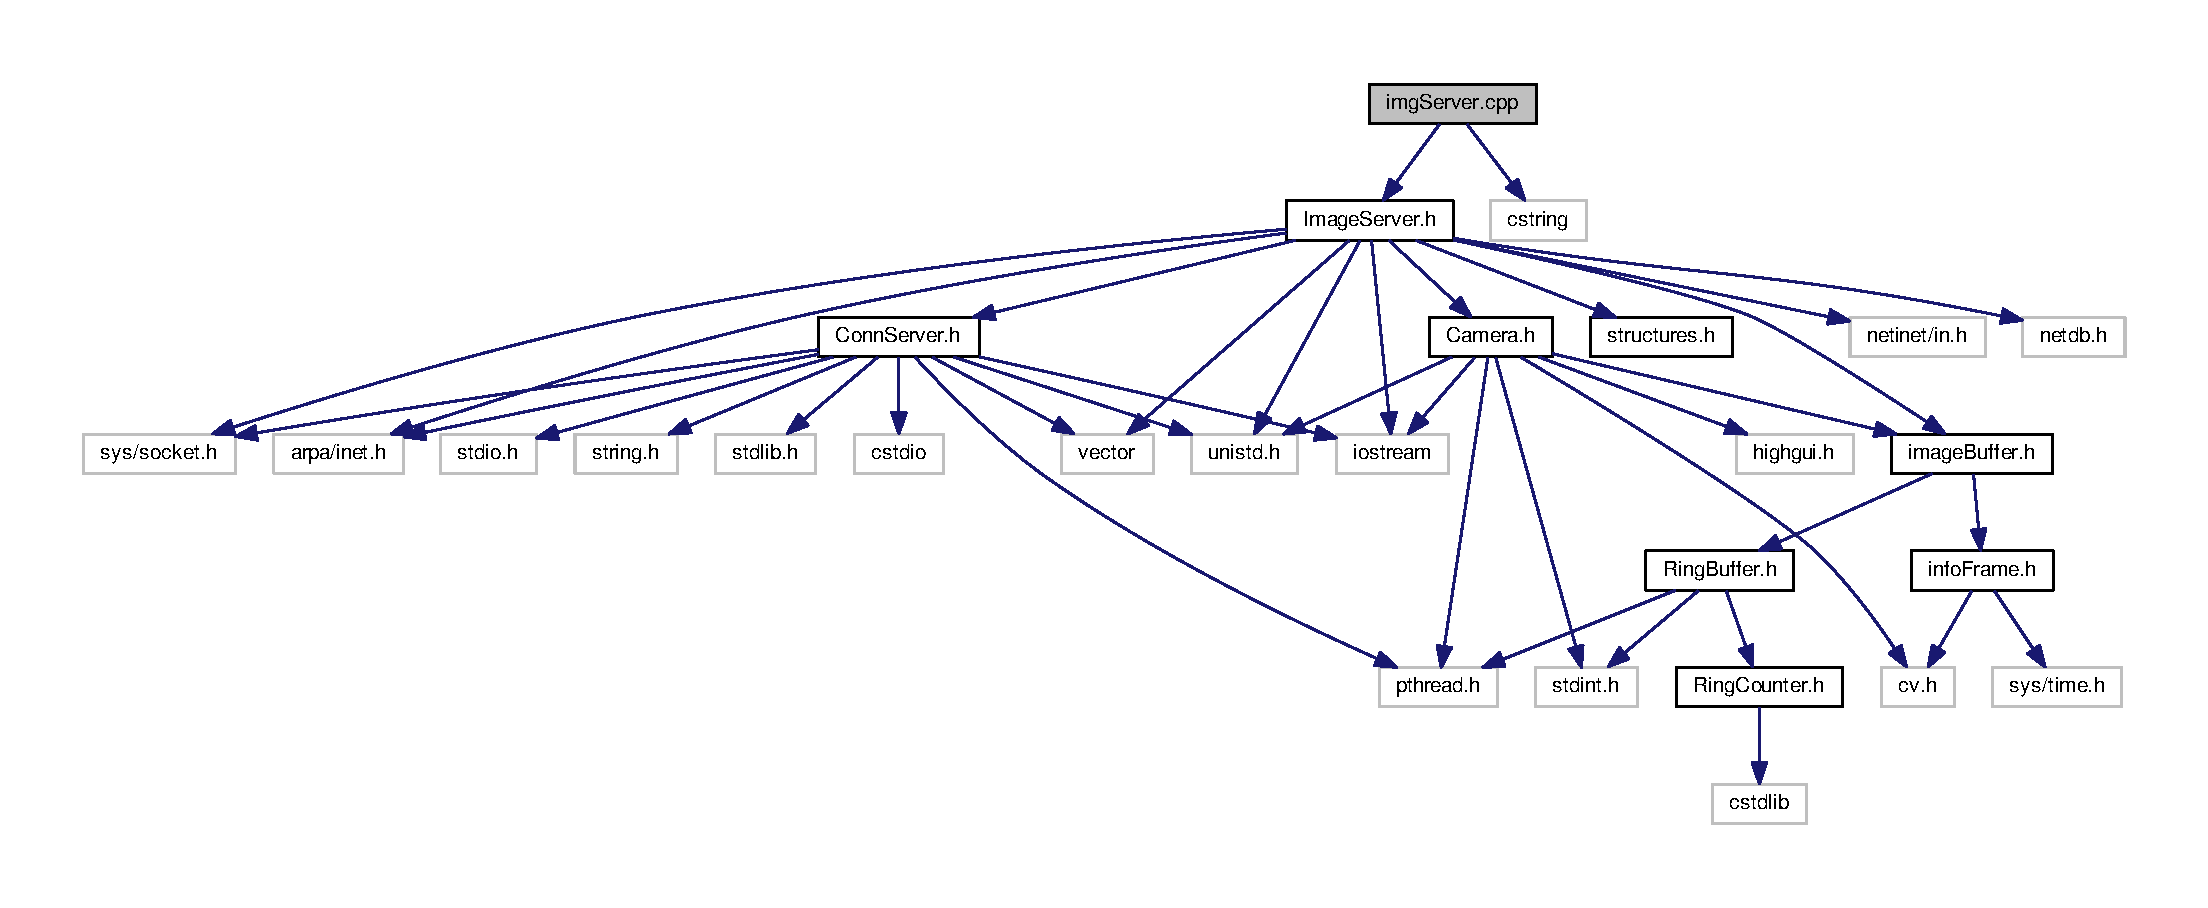
\includegraphics[width=350pt]{imgServer_8cpp__incl}
\end{center}
\end{figure}
\subsection*{Clases}
\begin{DoxyCompactItemize}
\item 
struct \hyperlink{structcornerData}{corner\+Data}
\begin{DoxyCompactList}\small\item\em Esta estructura contiene información de esquinas que se utiliza durante la captura de posiciones en la pantalla usando el raton. \end{DoxyCompactList}\end{DoxyCompactItemize}
\subsection*{Funciones}
\begin{DoxyCompactItemize}
\item 
void \hyperlink{imgServer_8cpp_a88e627368216f68e8ef03490c3802020}{dibuja\+Puntos} (Mat \&frame, Point2f $\ast$p, int n, Scalar color=Scalar(0, 0, 255))
\begin{DoxyCompactList}\small\item\em Esta función dibuja una lista de puntos en una imagen. \end{DoxyCompactList}\item 
void \hyperlink{imgServer_8cpp_ae6717d2afae0afa7db4f2fd217501ef4}{find\+Mapping} (int source, Point2f $\ast$v\+P, Mat \&H)
\begin{DoxyCompactList}\small\item\em Esta funcion se utiliza para obtener la información necesaria para rectificar las imagenes que el servidor va a capturar. La funcion captura imágenes de la fuente de video \char`\"{}source\char`\"{}, permite que usuario capture 4 coordenadas en la imagen utilizando el mouse, y a partir de esas cuatro coordenadas, calcula la transformación proyectiva que describe la transformación de esas 4 coordenadas al plano de la imagen. Se presume que el usuario va a elegir cuatro esquinas que yacen en un plano en la escena, y que la tranformación producida, permitira dedicar la atención de esa región únicamente. \end{DoxyCompactList}\item 
int \hyperlink{imgServer_8cpp_a3c04138a5bfe5d72780bb7e82a18e627}{main} (int argc, char $\ast$$\ast$argv)
\item 
void \hyperlink{imgServer_8cpp_a7c3f9a47b1a00ee638ccc26d9f00be4f}{on\+Mouse\+Event} (int event, int x, int y, int flags, void $\ast$data)
\begin{DoxyCompactList}\small\item\em Funcion que atiende evantos generados por el ratón. Esta funcion es invocada automáticamnete por el sistema cuando se registra usando la función set\+Mouse\+Callback de la biblioteca highgui. \end{DoxyCompactList}\end{DoxyCompactItemize}


\subsection{Documentación de las funciones}
\hypertarget{imgServer_8cpp_a88e627368216f68e8ef03490c3802020}{\index{img\+Server.\+cpp@{img\+Server.\+cpp}!dibuja\+Puntos@{dibuja\+Puntos}}
\index{dibuja\+Puntos@{dibuja\+Puntos}!img\+Server.\+cpp@{img\+Server.\+cpp}}
\subsubsection[{dibuja\+Puntos}]{\setlength{\rightskip}{0pt plus 5cm}void dibuja\+Puntos (
\begin{DoxyParamCaption}
\item[{Mat \&}]{frame, }
\item[{Point2f $\ast$}]{p, }
\item[{int}]{n, }
\item[{Scalar}]{color = {\ttfamily Scalar(0,0,255)}}
\end{DoxyParamCaption}
)}}\label{imgServer_8cpp_a88e627368216f68e8ef03490c3802020}


Esta función dibuja una lista de puntos en una imagen. 


\begin{DoxyParams}{Parámetros}
{\em Mat} & \&frame Imagen en donde se van a dibujar los puntos. \\
\hline
{\em Point2f} & $\ast$p Apuntador al arreglo de objetos de tipo Point2f que contiene las coordenadas de los puntos a dibujar. \\
\hline
{\em int} & n Cantidad de puntos a dibujar. \\
\hline
{\em Scalar} & color Objeto de tipo scalar que codifica en fomrto B\+G\+R el color de los puntos a dibujar. \\
\hline
\end{DoxyParams}


Definición en la línea 73 del archivo img\+Server.\+cpp.


\begin{DoxyCode}
74 \{
75 
76     \textcolor{keywordflow}{for} (\textcolor{keywordtype}{int} i=0;i<n; ++i)
77         circle(frame, Point((\textcolor{keywordtype}{int})p[i].x, (\textcolor{keywordtype}{int})p[i].y), 5, color);
78 \}
\end{DoxyCode}
\hypertarget{imgServer_8cpp_ae6717d2afae0afa7db4f2fd217501ef4}{\index{img\+Server.\+cpp@{img\+Server.\+cpp}!find\+Mapping@{find\+Mapping}}
\index{find\+Mapping@{find\+Mapping}!img\+Server.\+cpp@{img\+Server.\+cpp}}
\subsubsection[{find\+Mapping}]{\setlength{\rightskip}{0pt plus 5cm}void find\+Mapping (
\begin{DoxyParamCaption}
\item[{int}]{source, }
\item[{Point2f $\ast$}]{v\+P, }
\item[{Mat \&}]{H}
\end{DoxyParamCaption}
)}}\label{imgServer_8cpp_ae6717d2afae0afa7db4f2fd217501ef4}


Esta funcion se utiliza para obtener la información necesaria para rectificar las imagenes que el servidor va a capturar. La funcion captura imágenes de la fuente de video \char`\"{}source\char`\"{}, permite que usuario capture 4 coordenadas en la imagen utilizando el mouse, y a partir de esas cuatro coordenadas, calcula la transformación proyectiva que describe la transformación de esas 4 coordenadas al plano de la imagen. Se presume que el usuario va a elegir cuatro esquinas que yacen en un plano en la escena, y que la tranformación producida, permitira dedicar la atención de esa región únicamente. 


\begin{DoxyParams}{Parámetros}
{\em int} & source El identificador de la cámara que se va a utilizar.  Point2f $\ast$vp \\
\hline
\end{DoxyParams}


Definición en la línea 86 del archivo img\+Server.\+cpp.


\begin{DoxyCode}
87 \{
88     Point2f rP[4];
89     Mat Frame;
90     VideoCapture cap(source);
91     \hyperlink{structcornerData}{cornerData} cD;
92     \textcolor{keywordtype}{int} i = 0;
93 
94     \textcolor{keywordflow}{if} (!cap.isOpened())
95     \{
96         cerr << \textcolor{stringliteral}{"no se pudo abrir la cámara"} << endl;
97         \textcolor{keywordflow}{return};
98     \}
99 
100     namedWindow(\textcolor{stringliteral}{"Introduce esquinas"});
101     setMouseCallback(\textcolor{stringliteral}{"Introduce esquinas"}, \hyperlink{imgServer_8cpp_a7c3f9a47b1a00ee638ccc26d9f00be4f}{onMouseEvent}, (\textcolor{keywordtype}{void}*) &cD);
102     cD.\hyperlink{structcornerData_a961800bf60ff693820efbf7f4bc72788}{cont} = 0;
103     \textcolor{keywordflow}{while} (cD.\hyperlink{structcornerData_a961800bf60ff693820efbf7f4bc72788}{cont} < 4)
104     \{
105         cap >> Frame;
106         \textcolor{keywordflow}{if} (Frame.empty())
107             cerr << \textcolor{stringliteral}{"capturaPuntos: Error capturando el Frame"} << endl;
108         imshow(\textcolor{stringliteral}{"Introduce esquinas"}, Frame);
109         \hyperlink{imgServer_8cpp_a88e627368216f68e8ef03490c3802020}{dibujaPuntos} (Frame, cD.\hyperlink{structcornerData_a6d9e631d38806edbc61499fd4794baea}{crn}, cD.\hyperlink{structcornerData_a961800bf60ff693820efbf7f4bc72788}{cont});   
110         \textcolor{keywordflow}{if} (waitKey(30) >= 0)
111             \textcolor{keywordflow}{break};
112     \}
113     cvSetMouseCallback(\textcolor{stringliteral}{"Introduce esquinas"}, 0, 0);
114     \textcolor{keywordflow}{if} (cD.\hyperlink{structcornerData_a961800bf60ff693820efbf7f4bc72788}{cont} < 4)
115       cerr << \textcolor{stringliteral}{"La captura de puntos se aborto."} << endl;
116     \textcolor{keywordflow}{for} (\textcolor{keywordtype}{int} i=0;i<4;++i)
117         rP[i] = cD.\hyperlink{structcornerData_a6d9e631d38806edbc61499fd4794baea}{crn}[i];
118     cap.release();
119 
120     cout << \textcolor{stringliteral}{"Se capturaron los siguientes puntos:"} << endl;
121     \textcolor{keywordflow}{for} (i=0;i<4;++i)
122         cout << \textcolor{stringliteral}{"("} << rP[i].x << \textcolor{stringliteral}{", "} << rP[i].y << \textcolor{stringliteral}{")"} << endl;
123     H = getPerspectiveTransform(rP, vP);
124     destroyWindow(\textcolor{stringliteral}{"Introduce esquinas"});
125 \}
\end{DoxyCode}
\hypertarget{imgServer_8cpp_a3c04138a5bfe5d72780bb7e82a18e627}{\index{img\+Server.\+cpp@{img\+Server.\+cpp}!main@{main}}
\index{main@{main}!img\+Server.\+cpp@{img\+Server.\+cpp}}
\subsubsection[{main}]{\setlength{\rightskip}{0pt plus 5cm}int main (
\begin{DoxyParamCaption}
\item[{int}]{argc, }
\item[{char $\ast$$\ast$}]{argv}
\end{DoxyParamCaption}
)}}\label{imgServer_8cpp_a3c04138a5bfe5d72780bb7e82a18e627}


Definición en la línea 127 del archivo img\+Server.\+cpp.


\begin{DoxyCode}
128 \{
129          \textcolor{keywordtype}{int} \hyperlink{namespacetestClient_a1aadf525515ecfcf662c2aa51a503763}{port} = 8888, camId = 0;
130          \textcolor{keywordtype}{char} ipAddress[64] = \textcolor{stringliteral}{"127.0.0.1"};
131          Point2f vP[4], mP[4];
132      Mat Hrv, Hmv, Maze;
133 
134          Maze = 255 * Mat::ones(Size(640,480), CV\_8UC3);
135          \textcolor{keywordflow}{if} (\hyperlink{namespacetestClient_aad55a8f6b73a60a17d26dfc0d628f89a}{argc} < 2)
136          \{
137             cerr << \textcolor{stringliteral}{"Uso: imgServer camId ipAddress port Maze"} << endl;
138             \textcolor{keywordflow}{return} -1;
139      \}
140      \textcolor{keywordflow}{else}
141         camId = atoi(argv[1]);
142          \textcolor{keywordflow}{if} (\hyperlink{namespacetestClient_aad55a8f6b73a60a17d26dfc0d628f89a}{argc} > 2)
143          \{
144                         strncpy (ipAddress, argv[2], 63);
145                         \textcolor{keywordflow}{if} (\hyperlink{namespacetestClient_aad55a8f6b73a60a17d26dfc0d628f89a}{argc} > 3)
146                         \{
147                             port = atoi (argv[3]);
148                             \textcolor{keywordflow}{if} (\hyperlink{namespacetestClient_aad55a8f6b73a60a17d26dfc0d628f89a}{argc} > 4)
149                                 Maze = imread(argv[4]);
150                 \}
151         \}
152     
153      vP[0].x = 0; vP[0].y = 0;
154      vP[1].x = 639; vP[1].y = 0;
155      vP[2].x = 639; vP[2].y = 479;
156      vP[3].x = 0; vP[3].y = 479;
157      \hyperlink{imgServer_8cpp_ae6717d2afae0afa7db4f2fd217501ef4}{findMapping}(camId, vP, Hrv);
158      cout << \textcolor{stringliteral}{"Calculamos la Hrv como:"}<< endl << Hrv << endl;
159 
160      mP[0].x = 0; mP[0].y = 0;
161      mP[1].x = Maze.cols; mP[1].y = 0;
162      mP[2].x = Maze.cols; mP[2].y = Maze.rows;
163      mP[3].x = 0; mP[3].y = Maze.rows;
164      Hmv = getPerspectiveTransform(mP, vP);
165      cout << \textcolor{stringliteral}{"["} << Maze.cols << \textcolor{stringliteral}{", "} << Maze.rows << \textcolor{stringliteral}{"]"} << endl;
166      cout << \textcolor{stringliteral}{"Calculamos la Hmv como:"}<< endl << Hmv << endl;
167 
168          \hyperlink{classImageServer}{ImageServer} *imS = \textcolor{keyword}{new} \hyperlink{classImageServer}{ImageServer} (camId, port, ipAddress, &Hrv, &Hmv, &
      Maze);
169 
170          imS->\hyperlink{classImageServer_a60de64d75454385b23995437f1d72669}{start} ();
171 
172          sleep (3);                                                                             \textcolor{comment}{// wait for
       server to init}
173 
174          \textcolor{keywordflow}{do}
175          \{
176 
177          \}
178          \textcolor{keywordflow}{while} (\textcolor{keyword}{true});
179 
180          \textcolor{keywordflow}{return} 0;
181 \}
\end{DoxyCode}
\hypertarget{imgServer_8cpp_a7c3f9a47b1a00ee638ccc26d9f00be4f}{\index{img\+Server.\+cpp@{img\+Server.\+cpp}!on\+Mouse\+Event@{on\+Mouse\+Event}}
\index{on\+Mouse\+Event@{on\+Mouse\+Event}!img\+Server.\+cpp@{img\+Server.\+cpp}}
\subsubsection[{on\+Mouse\+Event}]{\setlength{\rightskip}{0pt plus 5cm}void on\+Mouse\+Event (
\begin{DoxyParamCaption}
\item[{int}]{event, }
\item[{int}]{x, }
\item[{int}]{y, }
\item[{int}]{flags, }
\item[{void $\ast$}]{data}
\end{DoxyParamCaption}
)}}\label{imgServer_8cpp_a7c3f9a47b1a00ee638ccc26d9f00be4f}


Funcion que atiende evantos generados por el ratón. Esta funcion es invocada automáticamnete por el sistema cuando se registra usando la función set\+Mouse\+Callback de la biblioteca highgui. 



Definición en la línea 52 del archivo img\+Server.\+cpp.


\begin{DoxyCode}
53 \{
54     \hyperlink{structcornerData}{cornerData} *cD;
55 
56     cD = (\hyperlink{structcornerData}{cornerData} *)data;
57     \textcolor{keywordflow}{if} (event == CV\_EVENT\_LBUTTONDOWN)
58     \{
59         cD->\hyperlink{structcornerData_a6d9e631d38806edbc61499fd4794baea}{crn}[cD->\hyperlink{structcornerData_a961800bf60ff693820efbf7f4bc72788}{cont}].x = x;
60         cD->\hyperlink{structcornerData_a6d9e631d38806edbc61499fd4794baea}{crn}[cD->\hyperlink{structcornerData_a961800bf60ff693820efbf7f4bc72788}{cont}].y = y;
61         cD->\hyperlink{structcornerData_a961800bf60ff693820efbf7f4bc72788}{cont}++;
62     \}
63 \}
\end{DoxyCode}

\input{Camera_8h}
\input{Client_8h}
\input{ConnServer_8h}
\input{imageBuffer_8h}
\input{ImageServer_8h}
\input{infoFrame_8h}
\input{RingBuffer_8h}
\input{RingCounter_8h}
\input{SockIO_8h}
\input{structures_8h}
\hypertarget{README_8md}{\section{Referencia del Archivo R\+E\+A\+D\+M\+E.\+md}
\label{README_8md}\index{R\+E\+A\+D\+M\+E.\+md@{R\+E\+A\+D\+M\+E.\+md}}
}

\hypertarget{remoteFrame_8py}{\section{Referencia del Archivo remote\+Frame.\+py}
\label{remoteFrame_8py}\index{remote\+Frame.\+py@{remote\+Frame.\+py}}
}
\subsection*{Clases}
\begin{DoxyCompactItemize}
\item 
class \hyperlink{classremoteFrame_1_1remoteFrame}{remote\+Frame}
\end{DoxyCompactItemize}
\subsection*{Namespaces}
\begin{DoxyCompactItemize}
\item 
 \hyperlink{namespaceremoteFrame}{remote\+Frame}
\end{DoxyCompactItemize}

\input{Camera_8cpp}
\input{Client_8cpp}
\input{ConnServer_8cpp}
\input{ImageServer_8cpp}
\input{SockIO_8cpp}
\hypertarget{testClient_8cpp}{\section{Referencia del Archivo test\+Client.\+cpp}
\label{testClient_8cpp}\index{test\+Client.\+cpp@{test\+Client.\+cpp}}
}
{\ttfamily \#include $<$Client.\+h$>$}\\*
{\ttfamily \#include $<$opencv2/core/core.\+hpp$>$}\\*
{\ttfamily \#include $<$opencv2/imgproc/imgproc.\+hpp$>$}\\*
{\ttfamily \#include $<$opencv2/highgui/highgui.\+hpp$>$}\\*
Dependencia gráfica adjunta para test\+Client.\+cpp\+:
\nopagebreak
\begin{figure}[H]
\begin{center}
\leavevmode
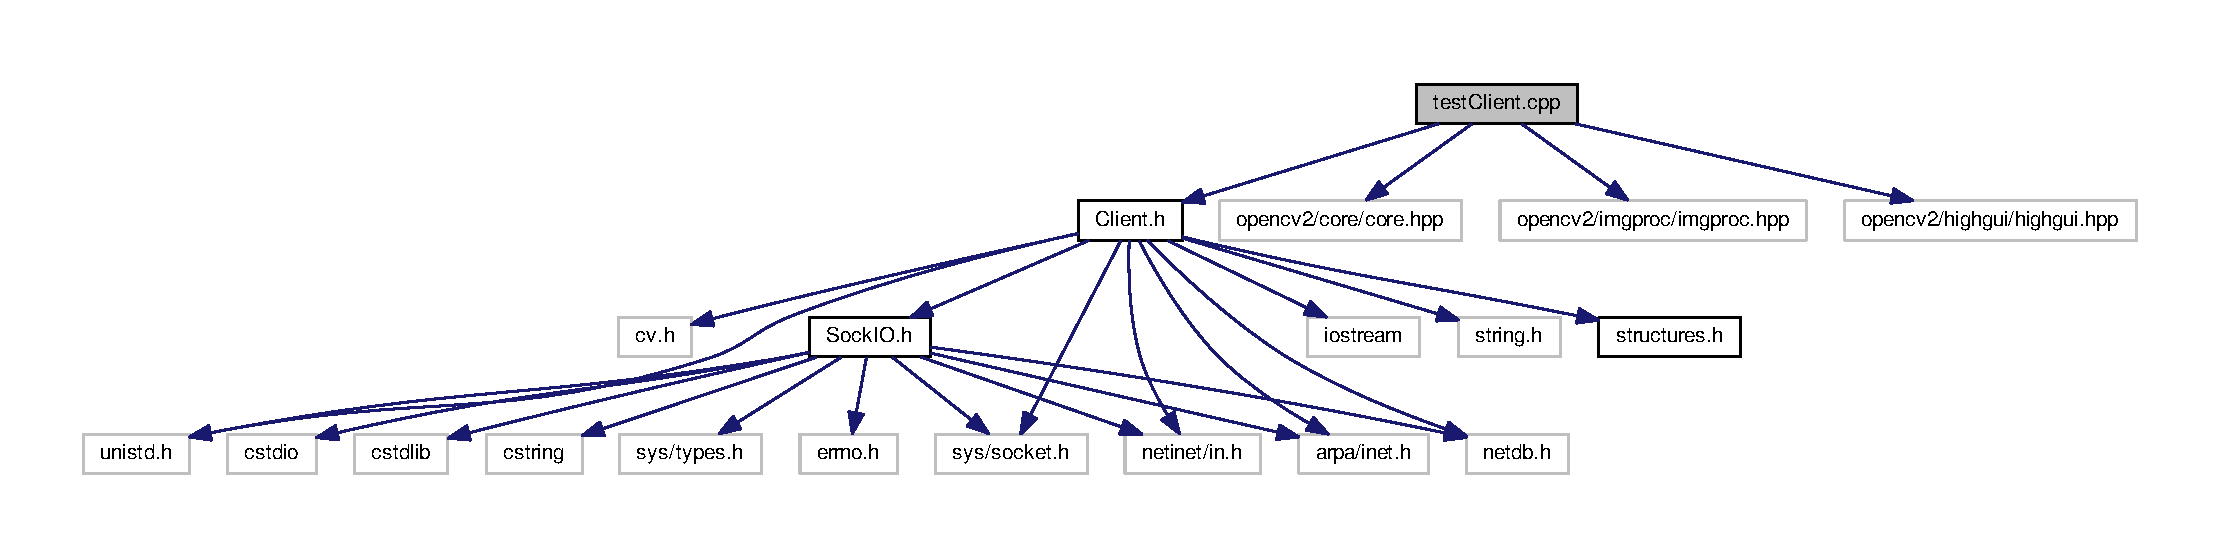
\includegraphics[width=350pt]{testClient_8cpp__incl}
\end{center}
\end{figure}
\subsection*{Funciones}
\begin{DoxyCompactItemize}
\item 
int \hyperlink{testClient_8cpp_a3c04138a5bfe5d72780bb7e82a18e627}{main} (int argc, char $\ast$$\ast$argv)
\end{DoxyCompactItemize}


\subsection{Documentación de las funciones}
\hypertarget{testClient_8cpp_a3c04138a5bfe5d72780bb7e82a18e627}{\index{test\+Client.\+cpp@{test\+Client.\+cpp}!main@{main}}
\index{main@{main}!test\+Client.\+cpp@{test\+Client.\+cpp}}
\subsubsection[{main}]{\setlength{\rightskip}{0pt plus 5cm}int main (
\begin{DoxyParamCaption}
\item[{int}]{argc, }
\item[{char $\ast$$\ast$}]{argv}
\end{DoxyParamCaption}
)}}\label{testClient_8cpp_a3c04138a5bfe5d72780bb7e82a18e627}


Definición en la línea 11 del archivo test\+Client.\+cpp.


\begin{DoxyCode}
12 \{
13          \textcolor{keywordtype}{int} \hyperlink{namespacetestClient_a1aadf525515ecfcf662c2aa51a503763}{port} = 8888;
14          \textcolor{keywordtype}{char} ipAddress[64] = \textcolor{stringliteral}{"127.0.0.1"};
15 
16          \textcolor{keywordflow}{if} (\hyperlink{namespacetestClient_aad55a8f6b73a60a17d26dfc0d628f89a}{argc} > 1)
17          \{
18                         strncpy (ipAddress, argv[1], 63);
19                         \textcolor{keywordflow}{if} (\hyperlink{namespacetestClient_aad55a8f6b73a60a17d26dfc0d628f89a}{argc} > 2)
20                                  port = atoi (argv[2]);
21          \}
22 
23          \hyperlink{classClient}{Client} *client = \textcolor{keyword}{new} \hyperlink{classClient}{Client} (port, ipAddress);
24          client->\hyperlink{classClient_a8381e13c2709536f7474cf6bdeb0ed8e}{connectSocket} ();
25 
26          Mat frame;
27          \textcolor{keywordflow}{while} (\textcolor{keyword}{true})
28          \{
29                         client->\hyperlink{classClient_a5ee9057ca3d53386f9979a058e6b2e86}{getFrame} (frame);
30                         imshow (\textcolor{stringliteral}{"rec"}, frame);
31                         \textcolor{keywordflow}{if} (waitKey (30) >= 0)
32                                  \textcolor{keywordflow}{break};
33          \}
34 
35 
36          \textcolor{keywordflow}{return} 0;
37 \}
\end{DoxyCode}

\hypertarget{testClient_8py}{\section{Referencia del Archivo test\+Client.\+py}
\label{testClient_8py}\index{test\+Client.\+py@{test\+Client.\+py}}
}
\subsection*{Namespaces}
\begin{DoxyCompactItemize}
\item 
 \hyperlink{namespacetestClient}{test\+Client}
\end{DoxyCompactItemize}
\subsection*{Variables}
\begin{DoxyCompactItemize}
\item 
string \hyperlink{namespacetestClient_aa723f31c9553b9750fa5b98615d0a8af}{address} = '127.\+0.\+0.\+1'
\item 
tuple \hyperlink{namespacetestClient_aad55a8f6b73a60a17d26dfc0d628f89a}{argc} = len(sys.\+argv)
\item 
tuple \hyperlink{namespacetestClient_aec8b285f81ee0dc468a6b86b4345e127}{img} = r\+F.\+get\+Frame()
\item 
\hyperlink{namespacetestClient_a09ad76b7b5cee406ff62ac1cdda80c27}{Mask} = None
\item 
int \hyperlink{namespacetestClient_a1aadf525515ecfcf662c2aa51a503763}{port} = 8888
\item 
tuple \hyperlink{namespacetestClient_a0be24333dfe323a6c01b9f452cc8b142}{r\+F} = remote\+Frame(address, port, Mask)
\end{DoxyCompactItemize}

%--- End generated contents ---

% Index
\newpage
\phantomsection
\addcontentsline{toc}{chapter}{Índice}
\printindex

\end{document}
